\documentclass{article}
\usepackage{graphicx}
\usepackage{geometry}
\usepackage{hyperref}
\usepackage{mathtools}
\usepackage{float}
\usepackage{minted}
\usepackage{xcolor}
\definecolor{LightGray}{rgb}{0.85,0.85,0.85}
\graphicspath{{./}}
\geometry{a4paper, portrait, margin = 1in}
\title{ROS Made Easy \\5: Gazebo}
\date{\today}
\author{Aniruddh K Budhgavi \\Enigma, IIIT-B}
\begin{document}
    \maketitle
    \section{Notes}
    \begin{enumerate}
        \item This tutorial was created for \textbf{ROS1 Melodic Morenia}
        on \textbf{Ubuntu 18.04 Bionic Beaver}, in \textbf{June 2020}.
        I expect them to become rapidly out of date. It is my hope
        that Team Enigma will continually maintain and update these tutorials.
        \item This tutorial assumes that you are running Ubuntu, and have at least an
        elementary grasp of Python 2.7 and C/C++ .
        \item All the code and the models for this tutorial are available at 
        \url{https://github.com/aniruddhkb/enigmatutorials}.
        \item The aim of this tutorial is to make you \emph{functional} in ROS, not to make you a master. For 
        that, look elsewhere.
        \item Ensure that you have RViz, TF2, the robot\_state\_publisher package and the joint\_state\_publisher
        and joint\_state\_publisher\_gui packages installed before proceeding further. You can install them 
        using the relevant \texttt{apt-get} commands. See \url{http://wiki.ros.org/rviz/UserGuide},
        \href{http://wiki.ros.org/tf2/Tutorials/Introduction%20to%20tf2}{this} and
        \href{https://answers.ros.org/question/346665/how-to-install-joint_state_publisher_gui-in-melodic-version-of-ros/}{this}.

        \item Ensure that you have \textbf{Meshlab} installed. Get it \href{https://snapcraft.io/install/meshlab/ubuntu}{here}.
    \end{enumerate}
    \section{Introduction}
        \begin{enumerate}
            \item Gazebo is an industry-standard robotics simulation tool. It integrates well with ROS, however, its compatibility with 
            the URDF file format is a little fuzzy -- it uses the SDF file format by default instead. To 
            make our URDF file Gazebo-compliant, we must add additional information to our URDF. The 
            most critical information we must provide are the \emph{inertial} and \emph{collision} properties 
            of our links.

            \item To add the collision properties, add something like the below code between
            your \texttt{link} tags:
            \begin{minted}[bgcolor=LightGray]{xml}
<collision>
  <geometry>
    <mesh filename="package://turret_bot/meshes/base.stl" scale="1 1 1"/>
  </geometry> 
</collision>
            \end{minted}
            Add the corresponding meshes to the links. Here, we are using the same mesh files as
            our \texttt{visual} meshes. This is fine for this example, however, typically, one uses 
            complex and visually appealing meshes for \texttt{visual} and greatly simplified meshes 
            (or even basic shapes) for the \texttt{collision} meshes.
            \item Next, we must add the \emph{inertial} properties to our model. To compute these 
            inertial properties, we use a software called \textbf{Meshlab}. You can get Meshlab from 
            \url{https://snapcraft.io/install/meshlab/ubuntu}.
        \end{enumerate}
    \section{Inertial properties}
        \subsection{Meshlab}
            \begin{enumerate}
                \item Launch Meshlab. You should see the following window:
                \begin{figure}[H]
                    \center
                    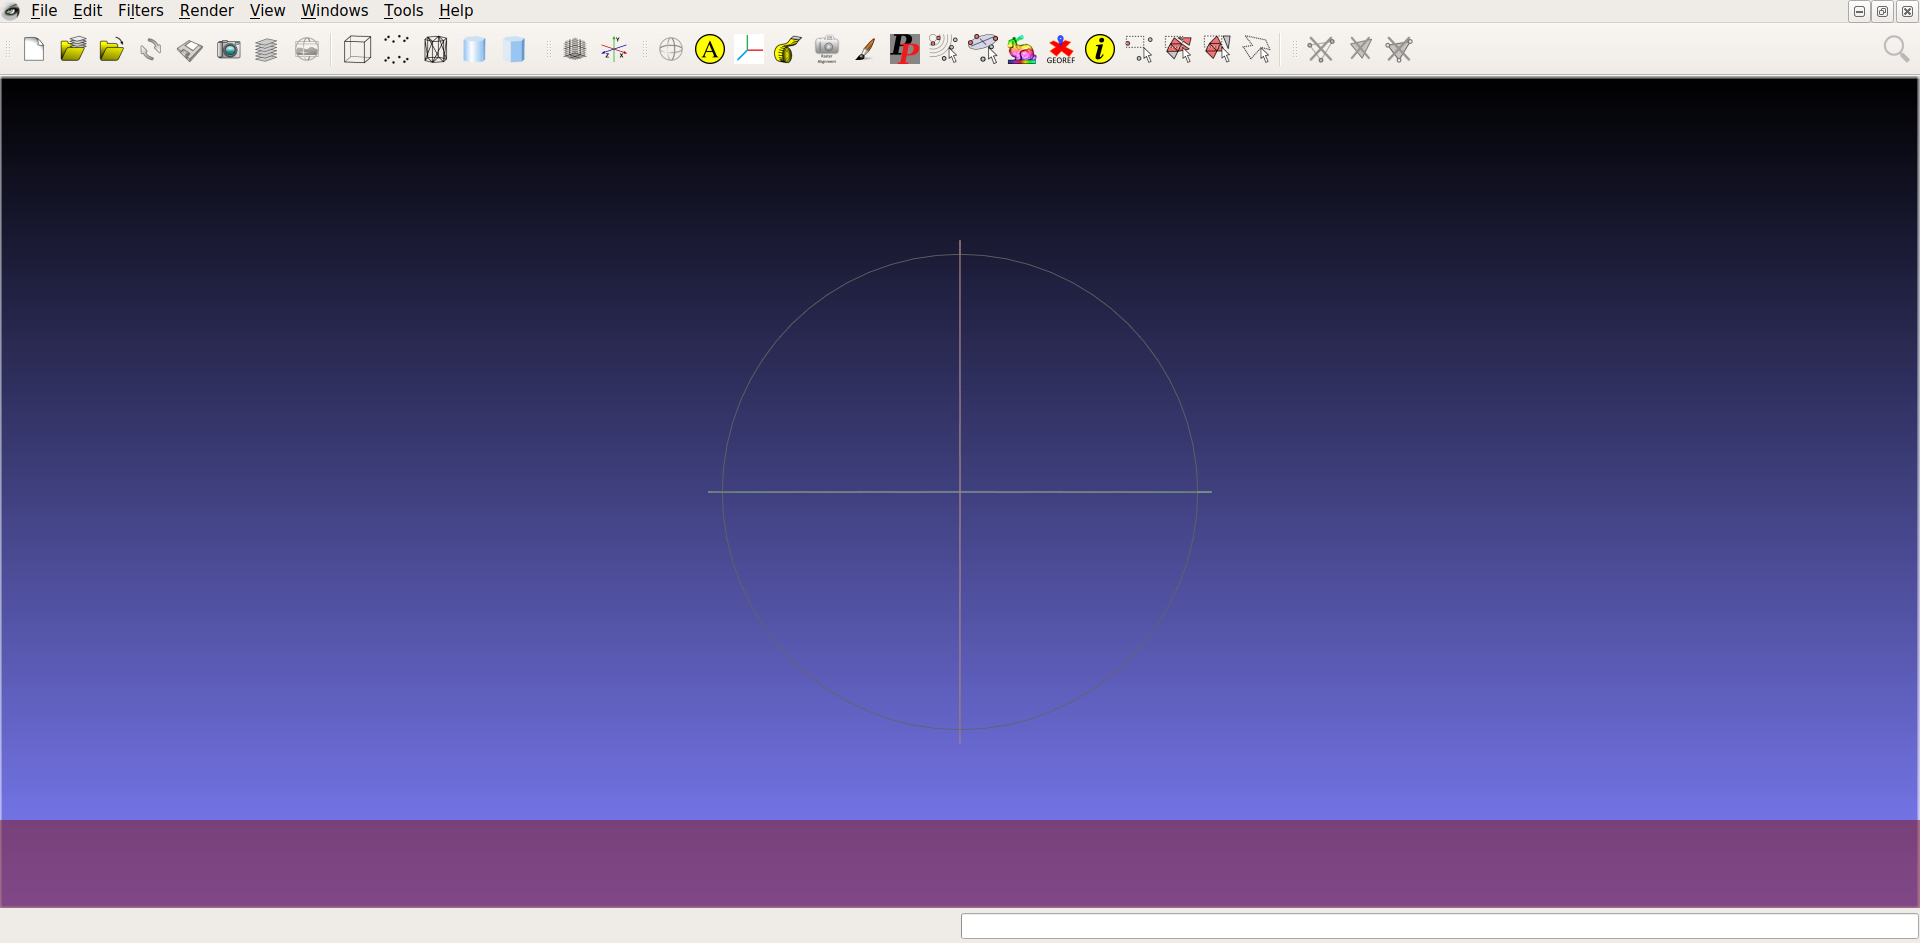
\includegraphics[width = \textwidth]{image_1.png}
                \end{figure}
                \item File -- Import Mesh -- base.stl . You should see:
                \begin{figure}[H]
                    \center
                    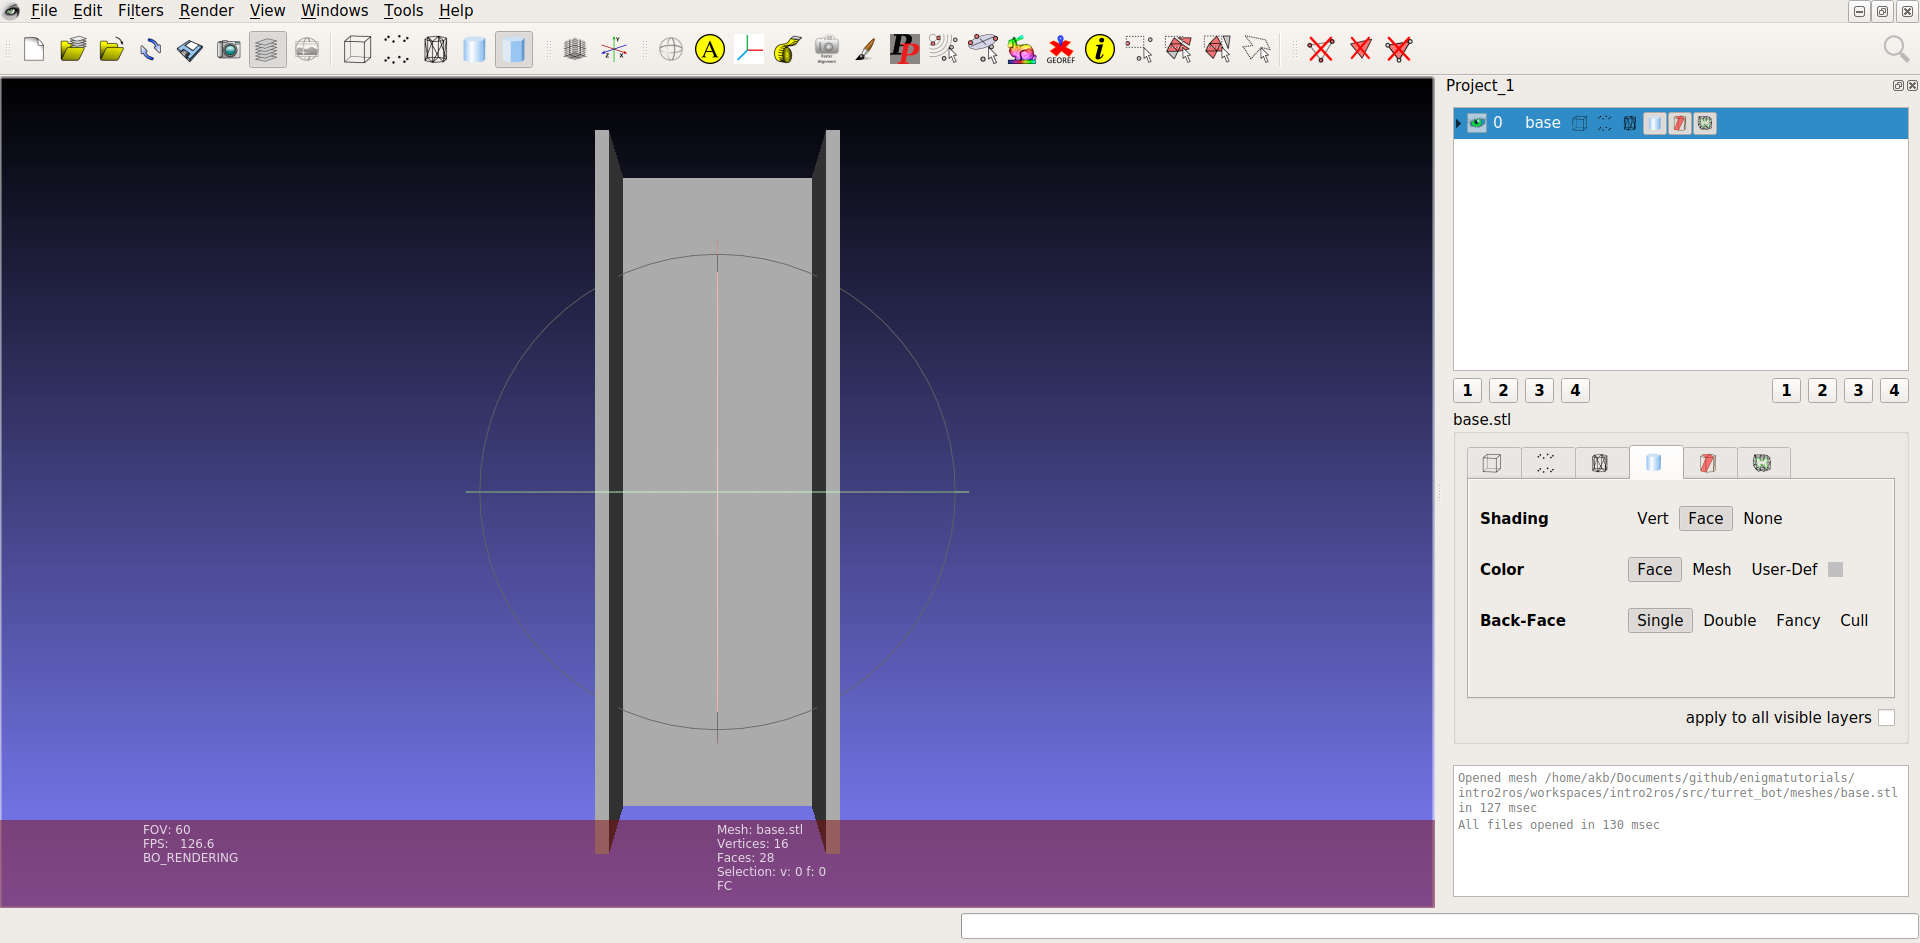
\includegraphics[width = \textwidth]{image_2.png}
                \end{figure}
                \item Filters -- Quality Measure and Computations -- Compute Geometric Measures. The output (bottom right corner box):
                \begin{minted}[bgcolor=LightGray]{python}
    Opened mesh base.stl in 127 msec
    All files opened in 130 msec
    Mesh Bounding Box Size 0.340000 1.000000 0.170000
    Mesh Bounding Box Diag 1.069813 
    Mesh Bounding Box min -0.170000 0.000000 -0.020000
    Mesh Bounding Box max 0.170000 1.000000 0.150000
    Mesh Surface Area is 1.345600
    Mesh Total Len of 42 Edges is 20.151415 Avg Len 0.479796
    Thin shell (faces) barycenter: 0.000000 0.500000 0.033118
    Vertices barycenter 0.000000 0.500000 0.070000
    Mesh Volume is 0.012800
    Center of Mass is 0.000000 0.500000 0.029844
    Inertia Tensor is :
    | 0.001101 0.000000 0.000000 |
    | 0.000000 0.000254 -0.000000 |
    | 0.000000 -0.000000 0.001286 |
    Principal axes are :
    | 0.000000 1.000000 0.000000 |
    | 1.000000 0.000000 0.000000 |
    | 0.000000 0.000000 1.000000 |
    axis momenta are :
    | 0.000254 0.001101 0.001286 |
    Applied filter Compute Geometric Measures in 42 msec
                \end{minted}
                Note down the \emph{mesh volume} and the \emph{center of mass}. Have a look at 
                the CoM value and ensure that the dimensions make sense. If they don't, you 
                probably exported the mesh in millimeters instead of meters.
                \item Filters -- Normals, Curvatures and Orientation -- Transform: Scale, Normalize
                -- X Axis: 10, Y Axis: 10, Z Axis: 10
                \item Run Compute Geometric Measures again. This time, note down the Inertia Tensor. 
                \textbf{This is not the final inertia tensor}(yet).
                \begin{minted}[bgcolor=LightGray]{python}
    Inertia Tensor is :
    | 110.117317 0.000000 0.000000 |
    | 0.000000 25.381306 -0.000000 |
    | 0.000000 -0.000000 128.597351 |
                \end{minted}
                \item Now, to get the real inertia tensor, multiply this matrix by the density of the material
                in \textbf{SI units} and $10^{-3}$. Further, to get the mass, multiply the volume you have above 
                by the density in SI units. I have written a short Jupyter notebook to assist me in these computations.
                It is available at the Github repo.
                \item Do this for all the links in your model. The reason we went through that step 
                of rescaling and rerunning the geometric measures computation is so that we could get 
                more decimal places in our calculation of the inertia tensor. For more information, see 
                \url{http://gazebosim.org/tutorials?tut=inertia&cat=build_robot}.
            \end{enumerate}
        \subsection{What is the inertia tensor?}    
            \begin{enumerate}
                \item At this stage, you must be having some questions about Meshlab and the inertia tensor.
                \item Recall that the rotational equivalent for mass is the moment of inertia about
                the axis of rotation.
                \item This definition of rotational inertia is useful, but is limited because it 
                is only applicable for a particular axis of rotation (ie a particular joint). In a 
                robot, a body may be simultaneously rotating about multiple axes in different directions.
                \item The inertia tensor is the answer to this dilemma. The inertia tensor is a generalization 
                of the concept of moment of inertia to three dimensions.
                \item More formally, the inertia tensor about a point about a set of axes is defined as:
                \[
I =     \begin{bmatrix}
        I_{xx} & I_{xy} & I_{xz} \\
        I_{yx} & I_{yy} & I_{yz} \\
        I_{zx} & I_{zy} & I_{zz}
        \end{bmatrix}
  =     \begin{bmatrix}
        \sum m_{i}(y_{i}^2 + z_{i}^2) & -\sum m_{i}x_{i}y_{i} &-\sum m_{i}x_{i}z_{i} \\
        -\sum m_{i}x_{i}y_{i} & \sum m_{i}(x_{i}^2 + y_{i}^2) & -\sum m_{i}y_{i}z_{i}  \\
        -\sum m_{i}x_{i}z_{i} & -\sum m_{i}y_{i}z_{i} & \sum m_{i}(x_{i}^2 + y_{i}^2)
        \end{bmatrix}                    
                \]
                \item The inertia tensor provided by Meshlab is about the specified axes about the center of mass.
                The assumption is that the body has a homogenous mass distribution of unit density, which is 
                why we need to multiply the density in SI units to get the correct answer.
                \item For more information, see \url{https://en.wikipedia.org/wiki/Moment_of_inertia}
            \end{enumerate}
        \subsection{The inertia tag}
            \begin{enumerate}
                \item Add something like the below code to each of your links:
                \begin{minted}[bgcolor=LightGray]{xml}
    <inertial>
        <origin xyz="0 0.5 0" rpy="0 0 0"/>
        <mass value="16"/>
        <inertia ixx="1.376" ixy="0" ixz="0" 
                 iyy="0.317" iyz="0" 
                 izz="1.607"/>
    </inertial>
                \end{minted}
                \item \texttt{origin} gives the center of mass. 
                \item \texttt{mass} is in kilograms (yes, that's a high mass. We usually use hollow bodies for this reason).
                \item \texttt{inertia} is the inertia tensor, expressed using the six numbers needed to specify it as given above.
            \end{enumerate}
    \section{Further steps}
        \subsection{Materials}
        Gazebo cannot use your \texttt{visual/material} tags. In order to 
        specify colors for the model, add the following between the \texttt{robot} tags 
        of the URDF.
        \begin{minted}[bgcolor=LightGray]{xml}
<gazebo reference="base">
<material>Gazebo/Green</material>
</gazebo>
        \end{minted}
        Add this for each of your links. For a list of Gazebo 
        materials, see \href{http://wiki.ros.org/simulator_gazebo/Tutorials/ListOfMaterials}{this} page.
        \subsection{Joints}
            \begin{enumerate}
                \item Ensure that your joint limits are correct. You'll get incorrect or unexpected behaviour otherwise. 
                If you wish to use position control later on, be sure that the joint limits are non-overlapping -- otherwise there 
                will be trouble.
                \item Add the following to each joint:
                \begin{minted}[bgcolor=LightGray]{xml}
    <dynamics damping="0.001" friction="0.001"/>
                \end{minted}
                \begin{enumerate}
                    \item \texttt{damping} is the viscous damping in Nm/(rad/s) or N/(m/s).
                    \item \texttt{friction} is the static frictional force in Nm or N.
                \end{enumerate}
            \end{enumerate}
        \newpage
        \subsection{The config file}
            In the package directory (very important -- not in a subfolder), create \texttt{model.config}:
            \begin{minted}[bgcolor=LightGray]{xml}
<?xml version="1.0"?>
<model>
    <name>turret_bot</name>
    <version>1.0</version>
    <sdf>urdf/turret_bot.urdf</sdf>
    <author>
        <name>Aniruddh K B </name>
        <email>aniruddhkb@gmail.com</email>
    </author>
    <description>
    A simple 2-dof robot for demonstration purposes.
    </description>
</model>          
            \end{minted}
            This is just a requirement for Gazebo.
        \subsection{The launch file}
            Create \texttt{launch/gazebo\_spawn.launch}:
            \begin{minted}[bgcolor=LightGray]{xml}
<?xml version="1.0"?>
<launch>
    <param name = "/robot_description" 
     textfile="$(find turret_bot)/urdf/turret_bot.urdf"/>
    <include file = "$(find gazebo_ros)/launch/empty_world.launch"/>
    <node name="urdf_spawner" pkg="gazebo_ros" type="spawn_model"
        args=" -unpause -urdf -model turret_bot 
               -param robot_description " respawn="false"/>
</launch>
            \end{minted}
        \subsection{Modify the environment variables}
            Add something like the following to your \texttt{.bashrc} :
            \begin{minted}[bgcolor=LightGray]{bash}
export GAZEBO_MODEL_PATH=/usr/share/gazebo-9/models
                         :<workspace-path>/src                
            \end{minted}
            This is so that Gazebo can find your models.
        \subsection{Fixing a bug}
            There is a bug in Gazebo which must be fixed before the first time you launch Gazebo. Open\\  
            \texttt{~/.ignition/fuel/config.yaml} and modify \texttt{https://api.ignitionfuel.org} to \\
            \texttt{https://api.ignitionrobotics.org}.
    \newpage 
    \section{Moment of truth}
        \begin{enumerate}
            \item Launch the launch file you created just now. If all goes well, you should see something like:
            \begin{figure}[H]
                \center
                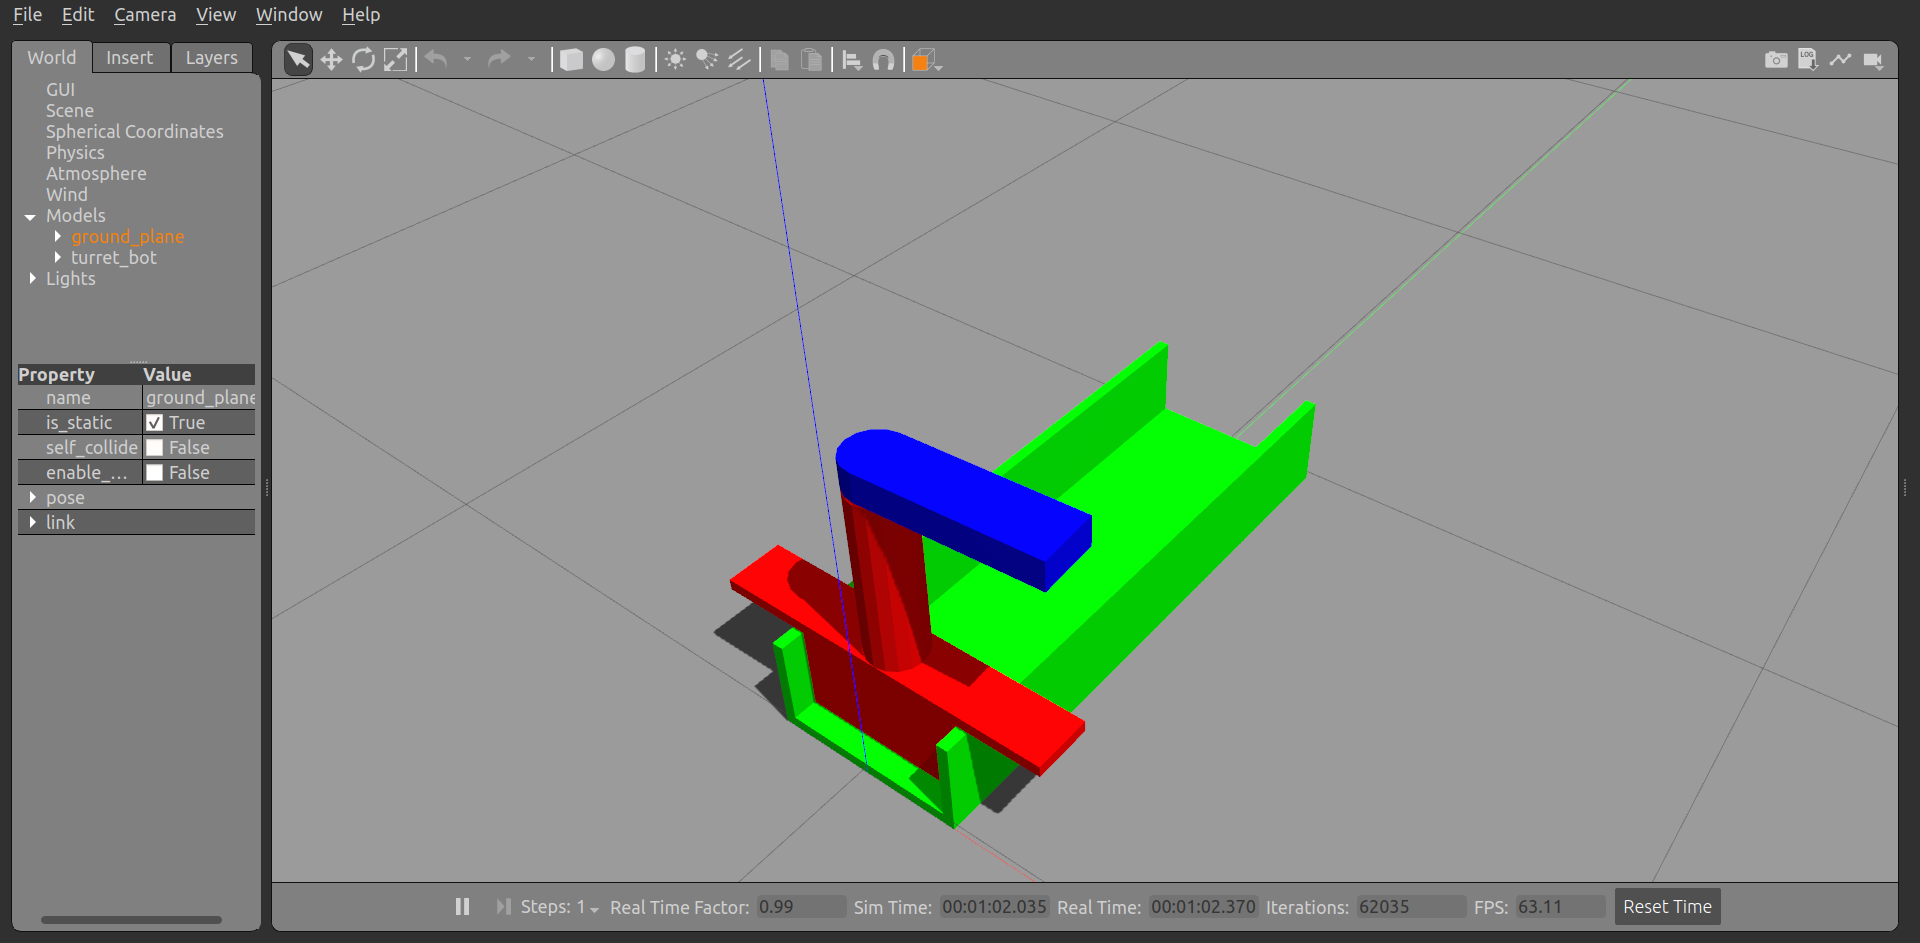
\includegraphics[width = \textwidth]{image_3.png}
            \end{figure}
            Use the three mouse buttons to navigate the world.
            \item View -- Moment of Inertia should show something like:
            \begin{figure}[H]
                \center
                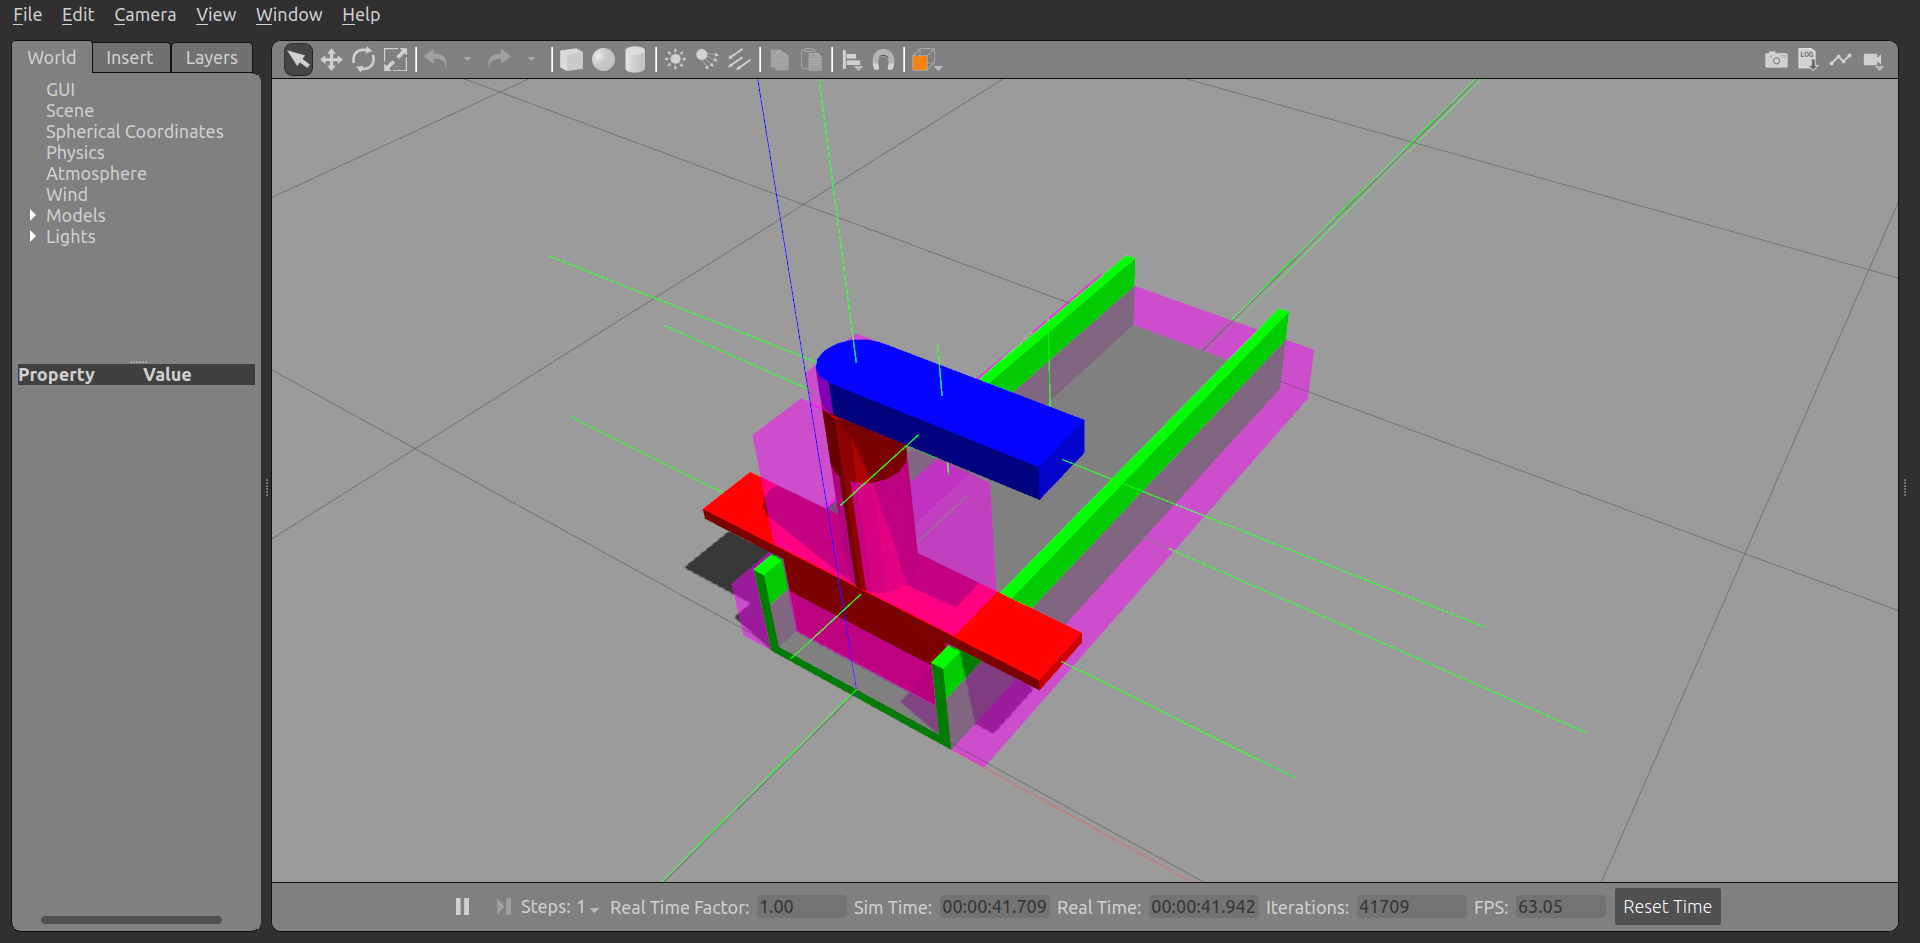
\includegraphics[width = \textwidth]{image_4.png}
            \end{figure}
            Those purple boxes are a representation of the inertia of those bodies. Ideally, they 
            should be pretty close (in terms of size) to the actual link size.

            \item Deactivate the inertia view, and open the right side pane by pulling from the right 
            of the window. Click on the model and choose "position". You should see:
            \begin{figure}[H]
                \center
                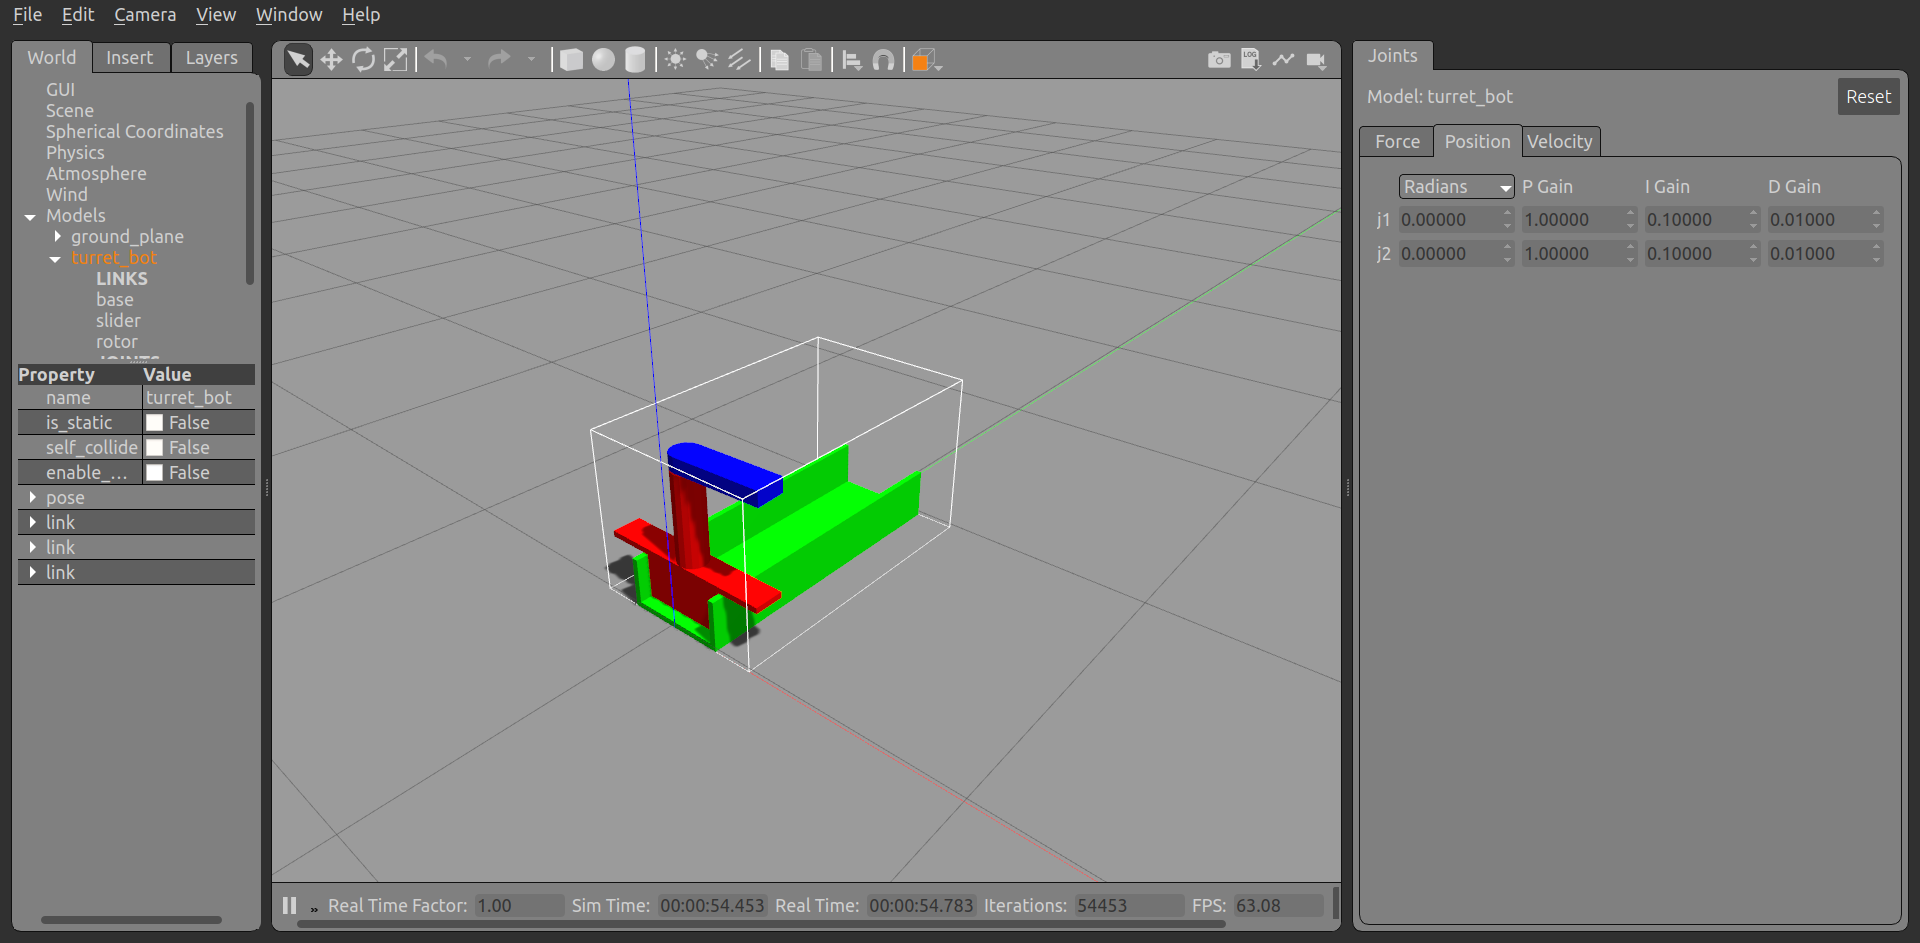
\includegraphics[width = \textwidth]{image_5.png}
            \end{figure}
            \item You can actuate the robot by giving position values to the joints. Be warned, however. The 
            position control is done through a PID feedback loop -- you'll have to tune the gains for P, I and D properly 
            in order to get good results. See \href{https://www.youtube.com/watch?v=HqrHktN-6TI}{this} video for the process I followed (it's fourteen minutes long, so you can skip along once you
            get a hang of it). \href{https://towardsdatascience.com/pid-controller-intro-26fda41aaa59}{This} is a good intro to PID tuning.
        \end{enumerate}
            
    \section{Looking ahead}
    You can now simulate a simple robot using Gazebo. Next time, we will use the \texttt{gazebo\_ros\_control} plugin to 
    control our simulated robot using ROS.
\end{document}